\documentclass{article}
\usepackage[utf8]{inputenc}
\usepackage{siunitx}
\usepackage{graphics}
\usepackage[american,siunitx]{circuitikz}
\usepackage{amsmath}
\usepackage{svg} 
\usepackage{booktabs}
\usepackage{float}
\usepackage{xparse, xfp}
\usepackage{graphicx} 
\usepackage{steinmetz}
\usepackage{multirow}
\usepackage{pdfpages}
\usepackage{adjustbox}
%\renewcommand{\thesubsection}{\thesection.\alph{subsection}}
\newcommand{\equal}{=}
\newcommand*\circled[1]{\tikz[baseline=(char.base)]{
    \node[shape=circle,draw,inner sep=1pt] (char) {#1};}}

\title{ECE 2101L\\Electrical Circuit Analysis II Laboratory\\\,\\Lab 12 and 13\\Maximum Power Transfer and Power Factor Correction\\\,\\Report\\}
\author{Choi Tim Antony Yung}
%\author{Choi Tim Antony Yung\\\,\\Willis Nguyen\\Phineas Cozmiuc}

\begin{document}

\clearpage\maketitle
\thispagestyle{empty}
\newpage
\setcounter{page}{1}


\section{Maximum power transfer}
\begin{figure}[H]
    \centering
        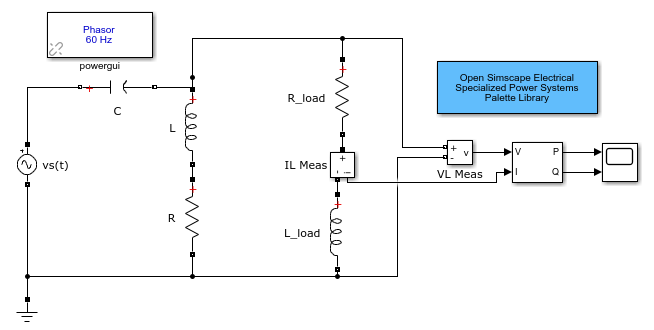
\includegraphics[width=\textwidth]{ECE2101L_Lab12_B1.png}
        \caption{Simulation of the circuit with MATLAB Simulink}
\end{figure}
\subsection*{Result}
C = \SI{220}{\micro\farad} for Partner 3
\begin{table}[H]
    \resizebox{\columnwidth}{!}{%
    \begin{tabular}{r|cc|cc|cc|c}
        \toprule
        \multirow{2}{*}{ Variant } & \multicolumn{2}{c|}{ Load Impedance $Z_L$ } & \multicolumn{2}{c|}{ Calc Power } & \multicolumn{2}{c|}{ Meas Power } & \multirow{2}{*}{ Error P, \% } \\
        & R, ohm & X, ohm & P, W & Q, VAR & P, W & Q, VAR & \\
        \midrule
        0.5 $Z_{L\_OPT}$ & 0.5278600 & 0.01718051 & NA & NA & 34.49 & 423.2 & NA \\
        0.8 $Z_{L\_OPT}$ & 0.8445760 & 0.02748882 & NA & NA & 237.7 & 2,916 & NA \\
        $Z_{L\_OPT}$ & 1.055720 & 0.03436103 & 687.8733 & NA & 687.9 & 8,440 & 0.00 \\
        1.2 $Z_{L\_OPT}$ & 1.266864 & 0.04123323 & NA & NA & 304.0 & 3,730 & NA \\
        1.5 $Z_{L\_OPT}$ & 1.583580 & 0.05154154 & NA & NA & 94.04 & 1,154 & NA \\
        \bottomrule
    \end{tabular} }
\end{table}


\subsection*{Analysis}
After changing the \SI{80}{\ohm} resistor to a \SI{330}{\ohm} resistor and changing the load inductor and resistor such that the power transfer to load is maximized, the maximum average power increased from 687.9\,W to 1502\,W. This is due to a decrease in load impedance and an increase of voltage of the load impedance.
\begin{figure}[H]
    \centering
        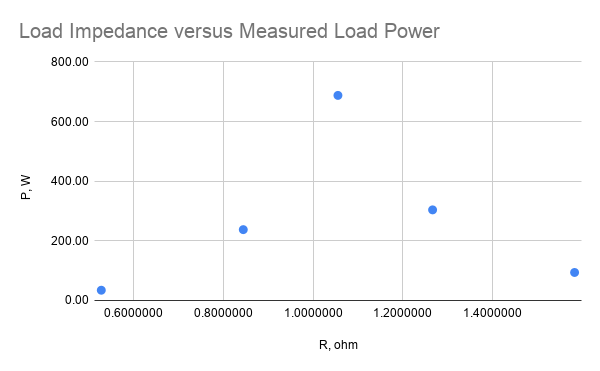
\includegraphics[scale=0.45]{ECE2101L_Lab12_B1_plot.png}
        \caption{Load Impedance versus Measured Load Power}
\end{figure}

\section{Circuit maximum gain and phase shift}

\subsection*{Result}
\begin{table}[H]
    \resizebox{\columnwidth}{!}{%
    \begin{tabular}{rc|cc|cc|cc}
        \toprule
        \multicolumn{2}{r|}{ Load PF } & Meas V1 & Meas I1 & Meas V2 & Meas I2 & Meas P & Meas Q \\
        & & RMS, V & RMS, A & RMS, V & RMS, A & loss, W & loss, VAR \\
        \midrule
        Original PF & 0.72 & 11000 & 4.911 & 229 & 219.4 & 2630 & 2700 \\
        Corrected PF & 0.95 & 11000 & 3.813 & 232.4 & 169.6 & 1980 & 2020 \\
        \bottomrule
        \end{tabular}  }
\end{table}

\subsection*{Analysis}
As seen in the above table, the current I1 and I2 decreased as the load draw less apparent power from the source. The voltage V2 decreased as the power dissipated from the wire decrease and the power dissipated from the load increase. As the current decreases, the power dissipated in wire decrease, hence the decrease in power loss.
\newpage

\begin{figure}[H]
    \centering
        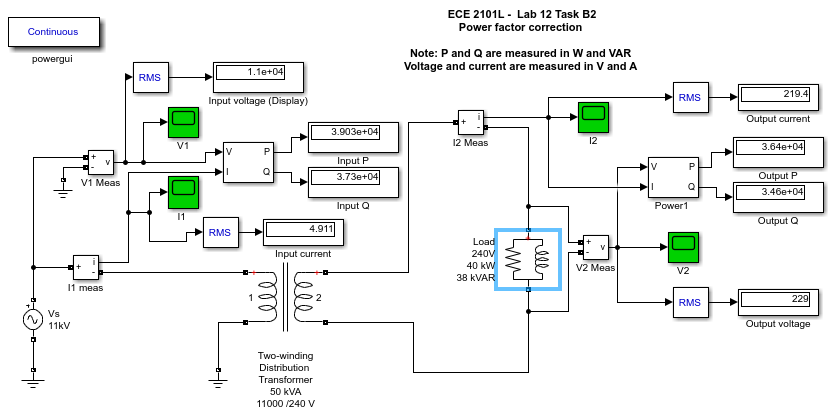
\includegraphics[width=\textwidth]{ECE2101L_Lab12_B2_0.72.png}
        \caption{Simulation of the circuit with original PF = 0.72}
\end{figure}
\begin{figure}[H]
    \centering
        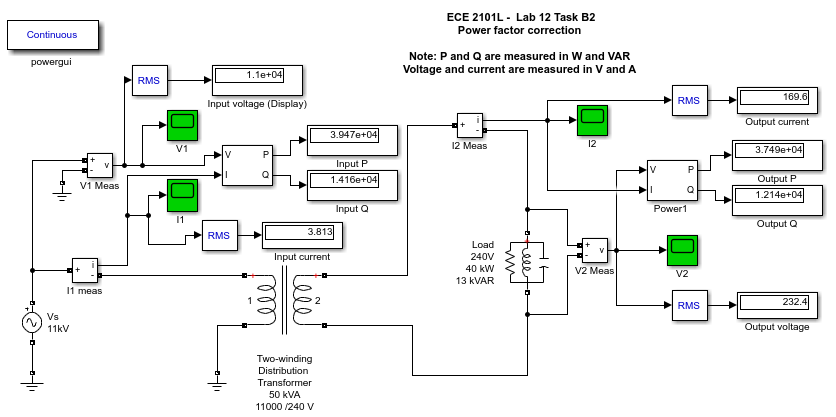
\includegraphics[width=\textwidth]{ECE2101L_Lab12_B2_0.95.png}
        \caption{Simulation of the circuit with corrected PF = 0.95}
\end{figure}

\end{document}

